\subsection{The NIC Packet Datapath}
\label{ssec:nic-datapath}
The NIC packet datapath (Figure~\ref{fig:nanoPU}a) processes packets as they enter and leave the network.
The centerpiece of the NIC packet datapath is an event-driven PISA pipeline~\cite{event-driven-pisa}. 
The original PISA architecture, proposed in the RMT chip~\cite{RMT} and later used by Tofino~\cite{tofino}, is designed for mostly-stateless match-action processing of packet headers; for example, for lookups, encapsulation, tunnels and telemetry.
Basic PISA only supports one type of event: the arrival of new packets. 
{\em Event-driven} PISA~\cite{event-driven-pisa} enhances the basic model to support other event types, such as packet drops, timers and state-dependent events. 
Section~\ref{ssec:nic-transport} describes how an event-driven PISA pipeline can directly support transport protocols in hardware, offloading per-packet processing from the CPU. 

The PISA pipeline also performs protocol processing: depending on the loaded P4 program~\cite{P4}, it might add and remove Ethernet, IP, VXLAN, GRE, INT~\cite{INT} and transport headers. 
We also program it to add or remove a small application-specific per-context header containing an IP address, a context ID, and the message length (\Cref{fig:app-headers}).

\begin{figure}
 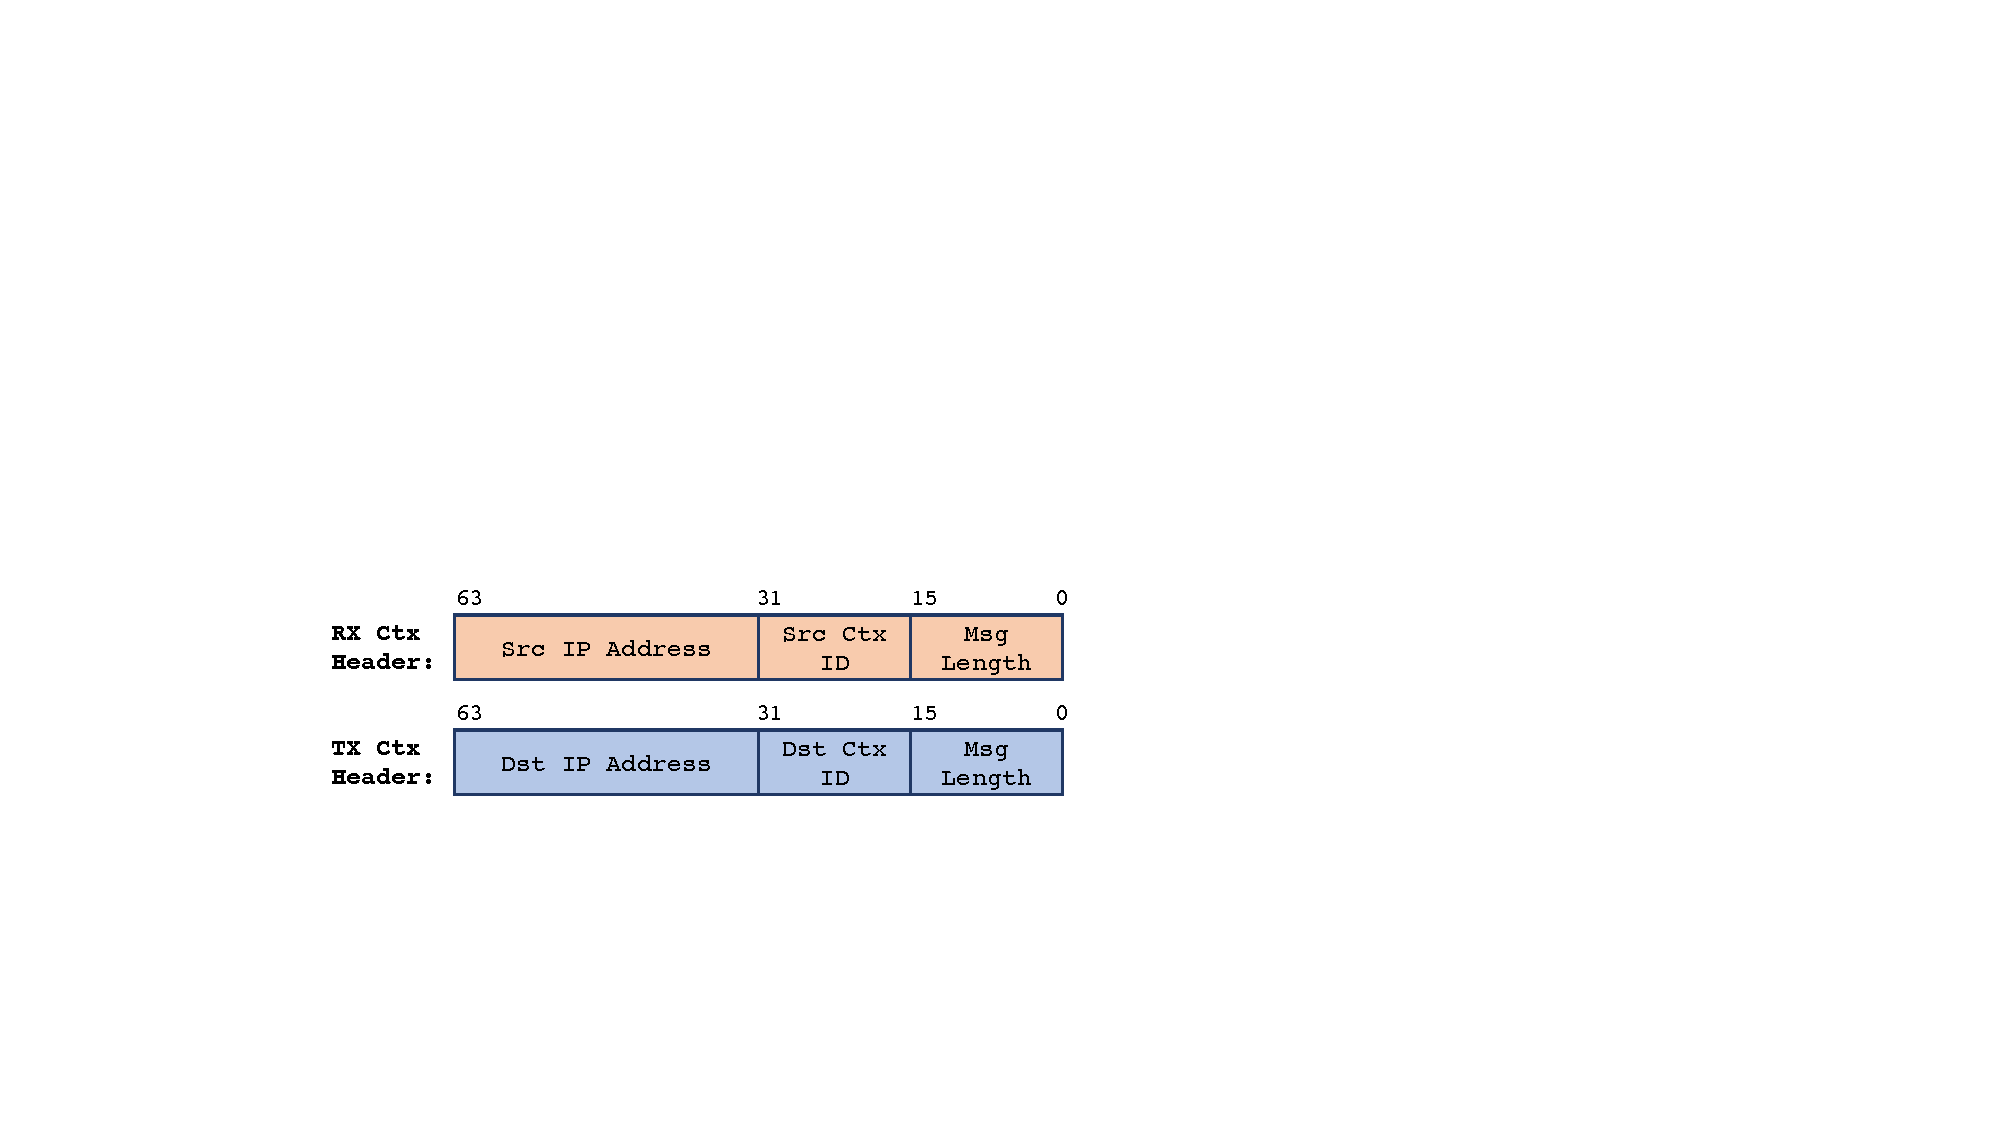
\includegraphics[width=0.95\linewidth]{./figures/ctx-hdr-fmt}
 \caption{NIC message (context) header formats.}
 \label{fig:app-headers}
\end{figure}

As others have noted, a P4-programmable PISA pipeline can also be used to accelerate some applications by offloading processing from the CPU (\eg, memory and disk caches~\cite{netcache}, load-balancers~\cite{silkroad}, consensus protocols~\cite{netchain} and firewalls~\cite{p4-firewall}). 
The L-NIC paper~\cite{lnic} describes how a PISA pipeline can accelerate nanoservices to search the Othello state-space.
